\section{Methodology}
\subsection{Outline}
This section will look into:
\begin{itemize}
	\item Mechanical Design:
	\item Electrical Design
	\item Instrumentation
	\item Software and Control Design
\end{itemize}

\subsection{Mechanical Design}
\subsubsection{Inverse Kinematics of a Stewart Platform}
This is the calculation of each leg length based on the desired position of the Stewart platform. 
For the Stewart platform, the translation $^{p}T_{b}$ from the base origin to the platform origin can be described with a single vector T = $(t_{x} t_{y} t_{z})^{T} $. The rotation of the platform can be denoted as $^{p}R_{b}$. Thus the following relationship for the frame of reference can be stated \cite{Eisele_2019}:
	\begin{ceqn}
	\begin{align}
	^{p}T_{b} = T
	\end{align}
	\end{ceqn}
	\begin{ceqn}
	\begin{align}
	^{p}R_{b} = R
	\end{align}
	\end{ceqn}
	\begin{ceqn}
	\begin{align}
	^{b}T_{p} =(^{p}T_{b})^{-1} =T^{-1}
	\end{align}
	\end{ceqn}
	\begin{ceqn}
	\begin{align}
	^{b}R_{p} = (^{p}R_{b})^{-1}
	\end{align}
	\end{ceqn} 
\begin{center}
	\begin{figure}[!h]
	\centering
	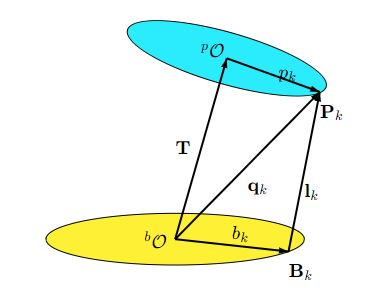
\includegraphics[width=0.4\linewidth]{Figures/servo2}
	\caption[Leg length]{Leg Length \cite{Eisele_2019}}
	\end{figure}
\end{center}
The leg length $l_{k}$ can therefore be found with:
\begin{ceqn}
\begin{align}
	l_{k} = P_{k} - B_{k} = T + R \times p \times R^{-1} - b_{k}
\end{align}
\end{ceqn}
Where,\\
$P_{k}$ - leg attachment on platform \\
$B_{k}$- leg attachment on base 
\subsubsection{Inverse Kinematics Using Rotational Servo Motors}
For a rod of fixed length d between servo horn anchor $H_{k}$ and platform anchor $P_{k}$.  $H_{k}$ has a distance h between the original base anchor and servo shaft $B_{k}$. The vector h is perpendicular to the servo shaft and is rotated by angle $\alpha_{k}$ when lifted from the horizontal line.
\begin{center}
	\begin{figure}[!h]
	\centering
	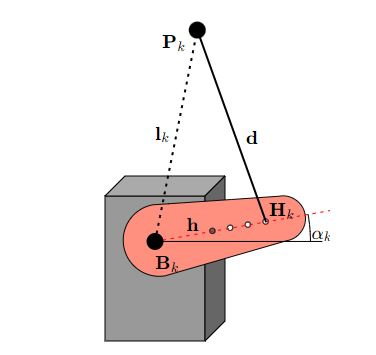
\includegraphics[width=0.4\linewidth]{Figures/servo}
	\caption[Servo angle]{Servo angle \cite{Eisele_2019}}
	\end{figure}
\end{center}
Further, looking from the top onto the base, each servo can be rotated by the angle $\beta_{k}$ in addition to its position $B_{k}$. The servo shaft $s_{k}$ moves in the x-y plane and is orthogonal to the vector h.
\begin{center}
	\begin{figure}[!h]
	\centering
	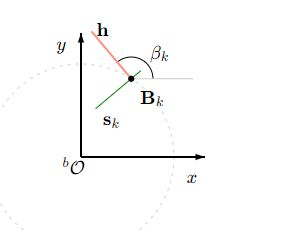
\includegraphics[width=0.4\linewidth]{Figures/servo1}
	\caption[Planar view]{Planar view \cite{Eisele_2019}}
	\end{figure}
\end{center}
The anchor $H_{k}$ can be calculated as we rotate around the z-axis with angle $\beta_{k}$ and  by $-\alpha_{k}$ around the y-axis to lift the servo horn which lies in the local x-axis \cite{Eisele_2019}.
\begin{ceqn}
\begin{align}
	H_{k} = B_{k} + R_{z}(\beta_{k}) R_{y}(-\alpha_{k})\begin{pmatrix}
	|h|\\ 0 \\ 0
	\end{pmatrix}
	\label{eq:myeqn2}
\end{align}
\end{ceqn}
\begin{ceqn}
 \begin{align}
	= B_{k} + |h|\begin{pmatrix}
	cos(\alpha_{k})cos(\beta_{k})\\
	 cos(\alpha_{k})sin(\beta_{k})\\
	  sin(\alpha_{k})
	\end{pmatrix}
	\label{eq:myeqn2}
\end{align}
\end{ceqn}
Carrying out the same procedure but with the servo arm when it is on the opposite side and we have:
\begin{ceqn}
\begin{align}
	H_{k} = B_{k} + R_{z}(\beta_{k}) R_{y}(\pi -\alpha_{k})\begin{pmatrix}
	-|h|\\ 0 \\ 0
	\end{pmatrix}
	\label{eq:myeqn2}
\end{align}
\end{ceqn}
\begin{ceqn}
	\begin{align}
	= B_{k} + |h|\begin{pmatrix}
	cos(\alpha_{k})cos(\beta_{k})\\
	 cos(\alpha_{k})sin(\beta_{k})\\
	  sin(\alpha_{k})
	\end{pmatrix}
	\label{eq:myeqn2}
\end{align}
\end{ceqn}
Squaring the lengths of h, d, $l_{k}$ we get the relationship:
\begin{ceqn}
	\begin{align}
		h^2 = (H_{k}-B_{k})^{T}(H_{k}-B_{k})
	\end{align}
\end{ceqn}
\begin{ceqn}
	\begin{align}
		d^2 = (P_{k}-H_{k})^{T}(P_{k}-H_{k})
	\end{align}
\end{ceqn}
\begin{ceqn}
	\begin{align}
		l_{k}^2 = (P_{k}-B_{k})^{T}(P_{k}-B_{k})
	\end{align}
\end{ceqn}
From the above relationships, further derivation and trigonometric substitutions are done to obtain the inverse kinematics used to calculate each servo angle. This is given as \cite{Eisele_2019}:
\begin{ceqn}
\begin{align}
	\alpha_{k} = sin^{-1}(\frac{g_{k}}{\sqrt{e_{k}^2+f_{k}^2}})-arctan2(f_{k}, e_{k})
\end{align}
\end{ceqn}
Where,
$$e_{k} = 2hl_{k}^{(z)} $$
$$e_{k} = 2h(cos(\beta_{k})I_{k}^{(x)}+sin({\beta_{k}})I_{k}^(y))$$
$$g_{k} = l_{k}^2 - (d^2 - h^2)   $$

\subsubsection{Actuation}
Two methods of actuation are popular with Stewart platforms:
\begin{itemize}
\item Linear actuators
\item Use of motors
\end{itemize}
Whereas linear actuators are relatively easy to control, they are very expensive. Thus the choice of motors.

\subsubsection*{Motor Selection}
One parameter was considered in our motor selection i.e. torque required. From the Autodesk Inventor design environment, the mass of the moving platform and mechanical couplings was 2.6kg. Each motor is supposed to move a minimum mass of 0.177kg. Using a servo horn of distance 45mm centre-to-centre, and Distance = $ \pi $ D, then:
\begin{ceqn}
\begin{align}
	Torque = (0.1777 \times 9.81)\times \frac{141.37}{1000} = 0.246 N\cdot m
\end{align}
\end{ceqn}
Motors of minimum torque of 0.2 N $\cdot m$ were considered. But for control considerations, only stepper motors and servo motors were shortlisted. Servo motor was considered over Stepper motor because they are cheaper. Also, we are only interested in 0 - 180 degrees positions.

The Servo motor \textbf{TowerPro MG995} is suitable for this project. The specifications provided by the manufacturer are as follows:

\begin{table}[!h]
\caption[Motor Specifications]{TowerPro MG995 Specifications}
\end{table}
\begin{center}
\begin{tabular}{|l|l|}
\hline
\textbf{Model}& TowerPro MG995\\
\hline
\textbf{Operating Voltage} & 4.8V - 6.6V\\
\hline
\textbf{Operating Speed @ 4.8V} & 0.20sec/60$^{\circ}$\\
\hline
\textbf{Operating Speed @ 6.6V}& 0.16sec/60$^{\circ}$\\
\hline
\textbf{Stall torque @ 4.8V} & 9.4 kg-cm or 0.94 N $\cdot$ m\\
\hline
\textbf{Stall torque @ 6.6V} & 11 kg-cm or 1.1 N $\cdot$ m\\
\hline
\end{tabular}
\end{center}
Prices range between \textbf{Ksh.700} and \textbf{Ksh.1400}

The previous servos used for the project were SG5010 which proved not to be able to handle the torque requirements of the platform, 
as a result the gears in those servos destroyed. The replacement of the servos with MG995 solved the problem due to the higher torque capacity.

\subsubsection{Finite Element Analysis}
A Finite Element Analysis was done on the Stewart platform design to determine its performance under given loads. The platform is going to be subjected to a force during wind tunnel testing. A maximum load of 50N is selected for the Finite Element Analysis. This could be more or less since models vary in size. The z-component of the force is considered. 
The mesh generated is shown in the figure \ref{fig:feamesh}.
\begin{center}
	\begin{figure}[H]
	\centering
	\includegraphics[width=0.75\linewidth]{Figures/FEA}
	\caption[Stewart platform mesh]{Stewart platform mesh}
	\label{fig:feamesh}
	\end{figure}
\end{center}
The rods/legs of the Stewart platform are subjected to axial forces which cause slight strains which can be used to obtain force and moment measurements during wind tunnel testing.
\clearpage
\begin{center}
\begin{table}[H]
\caption{Operating Conditions}
\centering
\end{table}
\begin{tabular}{|l|l|}
\hline
\textbf{Load Type} & \textbf{Force}\\
\hline
Magnitude & 50.0N\\
\hline
Vector X & 7.794N\\
\hline
Vector Y & -48.206N\\
\hline
Vector Z & 10.745N\\
\hline
\end{tabular}
\end{center}

\begin{center}
\begin{table}[!h]
\caption[FEA Setup]{Other FEA setup parameters}
\centering
\end{table}
\begin{tabular}{|l|l|}
\hline
Constraint & Fixed\\
\hline
Materials & Aluminium 6061\\
 & Stainless steel\\
\hline
Contacts & All bonded\\
\hline
Mesh& Avg element size: 0.1mm\\
& Minimum element size: 0.2mm\\
& Grading Factor: 1.50\\
& Maximum turn angle: 60 deg\\
\hline
\end{tabular}
\end{center}

\subsection{Strut}
The strut will go into the test section of the Wind tunnel. Consequently, it will be 
subjected to the flow forces in the wind tunnel. It has therefore been made of as small diameter as possible. 
A computational fluid dynamics test was done to ascertain the magnitude of drag force experienced and the effect that the strut
will have on the flow in the tunnel. The test was done using ANSYS.
\begin{center}
	\begin{table}[!h]
	\caption[CFD Setup]{CFD setup parameters}
	\centering
	\end{table}
	\begin{tabular}{|l|l|}
	\hline
	\textbf{Parameter} & \textbf{Value/Type}\\
	\hline
	Type of test & Fluid flow\\
	Type of fluid & air\\
	\hline
	Velocity & 10 - 50 m/s\\
	\hline
	\end{tabular}
	\end{center}
The speed of air flow in the wind tunnel is variable thus the simulation using speed between 10m/s and 50 m/s 
in steps of 10 m/s.

\subsubsection{Smoke Visualization System}
To implement streamline smoke lines in the wind tunnel, a smoke rake, which is an aerodynamically shaped
body (typically elliptical) featuring a row of tubes through which the smoke exits was designed. 
The CAD model was deigned using Autodesk Inventor and the rake was prepared for 3D printing at iPIC 
in JKUAT. The rake design is shown in figure \ref{smoke}.
\begin{center}
	\begin{figure}[H]
	\centering
	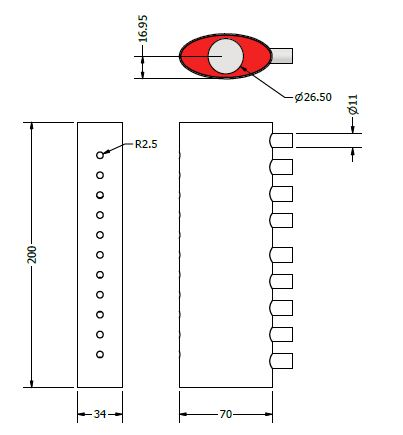
\includegraphics[width=0.7\linewidth]{Figures/smoke and rake.JPG}
	\caption[Smoke Rake]{Smoke rake design}
	\label{smoke}
	\end{figure}
\end{center}
The smoke emitting holes are 6mm in diameter and the air inlet holes are 5mm in diameter.
 20mm diameter hole on the lid (color coded red) shown in the  plan view is for metal pipe connection.

\subsubsection*{Smoke Rake and Pipe Assembly}
A metal pipe is used to provide rigid support to the smoke rake in the wind tunnel as well as placing it at the center
(vertically). A pipe of length 40mm and diameter 3/4"(19.05mm) is used. The pipe surface is roughed using a harcksaw in 
order to minimize any turbulence in the flow since it will be placed in the intake section. A plate of 10mm by 10mm by 1.5mm 
and two plumbing nuts are required to mount the pipe in the intake section. The smoke rake and pipe design is shown 
in figure \ref{pipe and rake}
\begin{center}
	\begin{figure}[H]
	\centering
	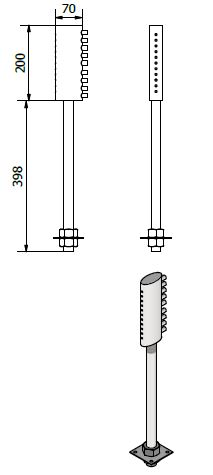
\includegraphics[width=0.25\linewidth]{Figures/pipe and rake.JPG}
	\caption[Pipe and rake]{Pipe and rake assembly design}
	\label{pipe and rake}
	\end{figure}
\end{center}

\subsection{Instrumentation}
\subsubsection{Design of the Force Sensor}
The force sensor module will be used to measure the force and moments from the aerodynamic loads applied on model being tested in the wind tunnel. The forces to be measured are the drag, lift and thrust as well as associated moments. For this subsystem two possible conceptual designs are to be considered:
\begin{itemize}
\item External force sensor
\item Stewart Platform as a force sensor
\end{itemize}
\subsubsection*{External Force Sensor}
In this case it would require at least 3 orthogonally positioned load cells measuring each force component. Each load cell would be mechanically linked to the model such that forces experienced on each axis are measured by each load cell as shown in figure \ref{fig:balex}. 
\begin{center}
	\begin{figure}[H]
		\centering
		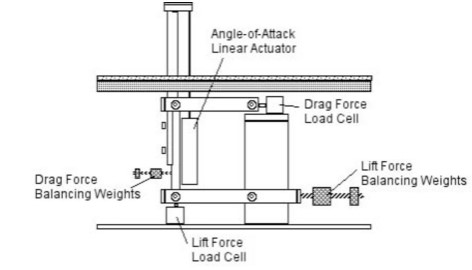
\includegraphics{Figures/modBal}
		\caption[Diagram of a force balance]{Diagram of a force balance \cite{post_force_2010}}
		\label{fig:balex}
	\end{figure}
\end{center}
This configuration is, however, bulky since it requires an additional external system for force measurements in addition to the Stewart platform for positioning the model. This is however complemented by the simplicity in calibration of the load cells and does not require a complex force transformation matrix and other issues with force amplification created by the use of an integrated system.
\subsubsection*{Stewart Platform as a force sensor}
In this configuration the Stewart platform legs are used as force sensors by attaching strain gauges on the legs of platform. Similar work has been done by \cite{ferreira2015design} without the use of actuators as is proposed in this project. Using the Stewart platform as a force sensor requires the actuators to be locked with zero degrees of freedom.

Four strain gauges are required for each leg for a full Wheatstone bridge configuration. 
\begin{center}
	\begin{figure}[H]
		\centering
		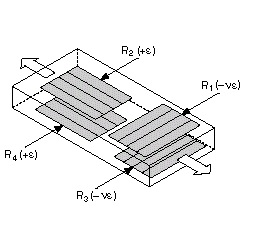
\includegraphics{Figures/loadConf}
		\caption[Strain Gauge Configuration]{Strain Gauge Configuration \cite{noauthor_measuring_nodate}}
		\label{strain}
	\end{figure}
\end{center}
In this case, as shown in figure \ref{strain}, the load cells are able to measure the axial strain on each leg. R1 and R3 are active strain gauges measuring the compressive Poisson effect (–νe). R2 and R4 are active strain gages measuring the tensile strain (+e). The output generated from the Wheatstone bridge is then amplified and read to determine the strain on each leg.
In the case of this project, a full bridge strain gauge sensor with each strain gauge orthogonally positioned allowing for elimination of noise and measurement of the strain axially on each rod is used.

\subsubsection*{Force transformation matrix} 
The forces experienced at the top of the platform are distributed between the 6 legs and as result, a force transformation matrix is required to resolve the forces applied on each axis as measured by each load cell on each leg. 

The forces experienced by the legs can be expressed as:
\begin{ceqn}
\begin{align}
	\begin{Bmatrix}
		\vec{F}_e \\
		\vec{M}_e \\
	\end{Bmatrix} = [H]\{F\}
\end{align}
\end{ceqn}

Where 
\begin{itemize}
\item $\vec{F}_e $ - external force applied to the platform
\item $\vec{M}_e$ - external moment applied to the platform
\item H - transformation matrix which relates measured forces and applied forces
\item F - axial force
\end{itemize}  
The derivation has been done and is presented in the appendix.

\subsubsection*{Bonding strain gauges}
The bonding of the strain gauges to the rods followed the following process:
\begin{itemize}
	\item Roughing of boding surface using sand paper
	\item Cleaning bonding surface using acetone
	\item Apply super glue to bonding surface and bond the strain gauge to the rod
	\item Apply resin (araldite) on the bonded strain gauge to protect the strain gauge from damage
	\item Solder jumper wires to the leads on the strain gauge as shown in \ref{fig:strain_bond}.
	\item Finally cover the assembly with heat shrinkable tubing 
\end{itemize}
\begin{center}
	\begin{figure}[H]
		\centering
		\includegraphics[width=0.7\linewidth]{Figures/strain_bond}
		\caption[Strain gauge bonding process]{Strain gauge bonding process}
		\label{fig:strain_bond}
	\end{figure}
\end{center}

\subsection{Velocity Measurement}
An important part in wind tunnel measurements is the measure of pressure at specific points in the wind tunnel and computing the corresponding air speed. This is achieved by the use of a pitot probe. 
\begin{center}
\begin{figure}[H]
\centering
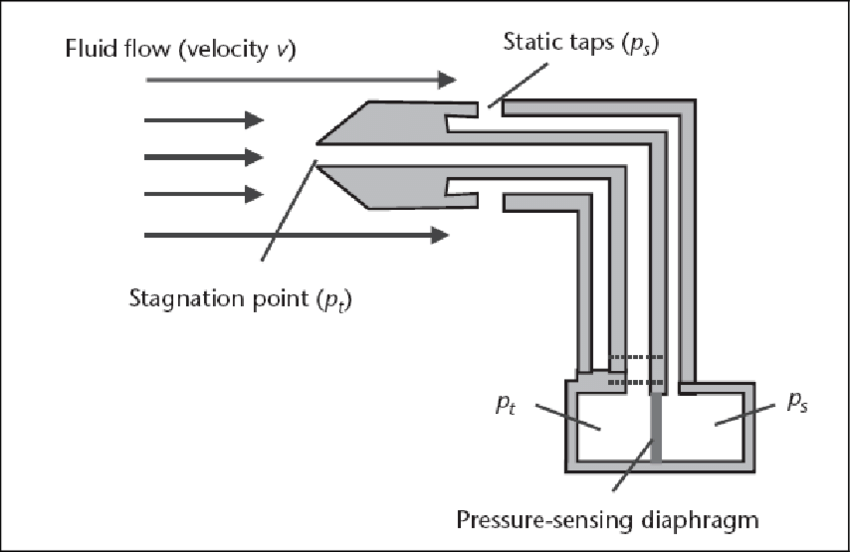
\includegraphics[width=0.6\linewidth]{Figures/pitot}
\caption[Pitot-static tube]{Pitot-static tube \cite{viquerat_continuous_2006}}
\end{figure}
\end{center}
For steady flow of an incompressible fluid for which viscosity can be neglected, the fundamental equation has the form\cite{viquerat_continuous_2006}:

\begin{ceqn}
	\begin{align}
	v = \sqrt{\frac{2(P_{0} - P)}{\rho}}
\end{align}
\end{ceqn}

Where V is the speed of the fluid, $P_{0}$ is the total, also called the stagnation, pressure at that point of measurement, and P is the static pressure at the same point.
                                                                                                                                                           
\begin{center}
\begin{figure}[H]
\centering
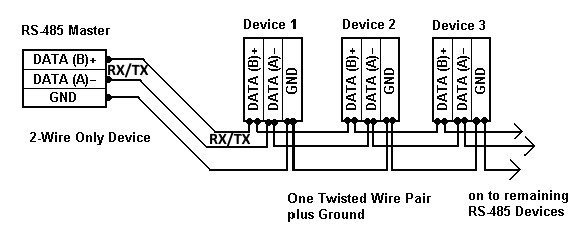
\includegraphics{Figures/modbus}
\caption[RS485 communication]{RS485 communication}
\label{fig:rs485}
\end{figure}
\end{center}
The module communicates to the microcontroller using a TTL to RS485. Each module is individually addressable further simplifying the interface as shown in figure \ref{fig:rs485}. 
The protocol allows for long distance serial communication and interface with multiple devices on the same bus.

Three pitot probes are to be used in the wind tunnel i.e. in the test section, intake and diffuser sections.
\begin{center}
	\begin{figure}[H]
	\centering
	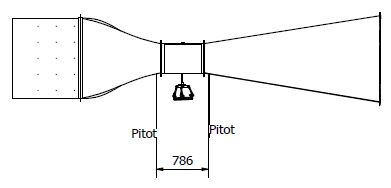
\includegraphics{Figures/wt and pitot.JPG}
	\caption[Pitot setpu]{Pitot setup in the intake and diffuser}
	\label{pitot loc}
	\end{figure}
\end{center}
Pitot location in the intake is exactly at the beginning of the test section and pitot location in the diffuser
is exactly at the end of the test section as shown in figure \ref{pitot loc}.

\subsection{Electrical Design}
This section looks at the required electrical connections to make the system functional and interface with the control unit.
\subsubsection{Printed Circuit Board Design}
This section looks at the design of the circuits used to power and get readings from the sensors and control the actuators.

\subsubsection{Microcontroller}
The main requirement for this is the need for wireless communication via WIFI and large number of I/O interface at cost effective rate. This brings down the options to the ESP32 and Raspberry Pi RP2040. Both are dual core devices which are feature rich however the raspberry rp2040 only has 28 I/O pins while the ESP32 has 34 pins and due to this the ESP32 was chosen. 
\begin{center}
	\begin{figure}[H]
	\centering
	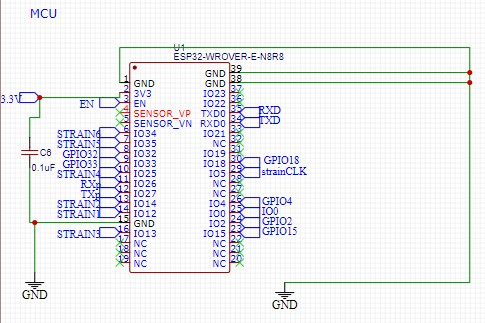
\includegraphics[width=0.7\linewidth]{Figures/mcu}
	\caption[Microcontroller]{Microcontroller}
	\end{figure}
\end{center}
\subsubsection{Power Supply}
The power supply chosen is an AC/DC power converter since the highest voltage required is 12 volts. This is also used as the highest power supply to the PCB.

Both 5 and 3.3 volts are required in the PCB for other peripherals. To this end, a buck converter and linear converter are used for 5 ad 3.3 volts respectively.

\begin{center}
	\begin{figure}[H]
	\centering
	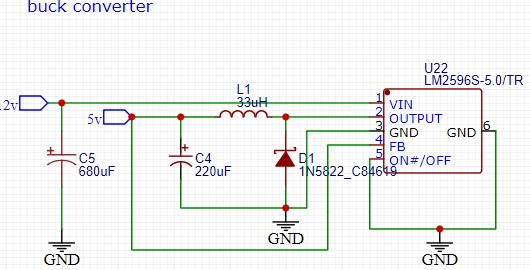
\includegraphics{Figures/buck}
	\caption[Buck converter]{Buck Converter 12V to 5V}
	\end{figure}
\end{center}

\begin{center}
	\begin{figure}[H]
	\centering
	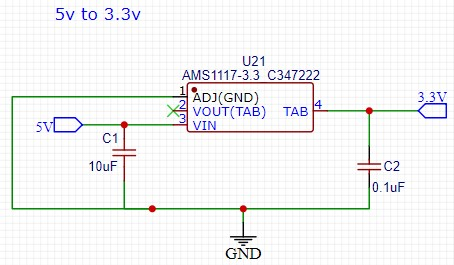
\includegraphics{Figures/5233}
	\caption[Linear Voltage Converter]{Linear level converter 5V to 3.3v}
	\end{figure}
\end{center}
The linear converter dissipates the energy loss though heat while buck converter is through switching.

\subsubsection{Servo Control}
Since the microcontroller used (ESP32) is based on 3.3V logic. There is a need for 5V logic to control the servos and thus a bidirectional logic level converter is utilized which leverages an internal drain N-channel MOSFET. 
\begin{center}
	\begin{figure}[H]
	\centering
	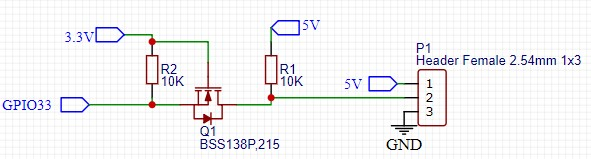
\includegraphics{Figures/logik}
	\caption[Bidirectional Logic Level converter]{Bidirectional Logic Level converter}
	\label{fig:logik}
	\end{figure}
\end{center}
The configuration designed is shown in figure \ref{fig:logik}

\subsubsection{Force measurement Circuit}

The output excitation of the Wheatstone bridge needs to be amplified as it results in low outputs. An analogue to digital converter is also required for the analogue to digital converter. Some considerable options are the HX711 or the AD7193 converters which may be used as digital to analogue converters. The AD7193 is designed for high precision and has a delta sigma filter to remove noise from measurements.  However, the AD7193 was not used due to it's high cost compared to the HX711 regardless of the advantage it offers with serial peripheral Interface communication allowing for multiple modules on the same bus.

The connection of the AD7193 to the microcontroller will be via Serial Peripheral Interface (SPI). The configuration is as shown in figure \ref{spi}:
\begin{center}
\begin{figure}[H]
\centering
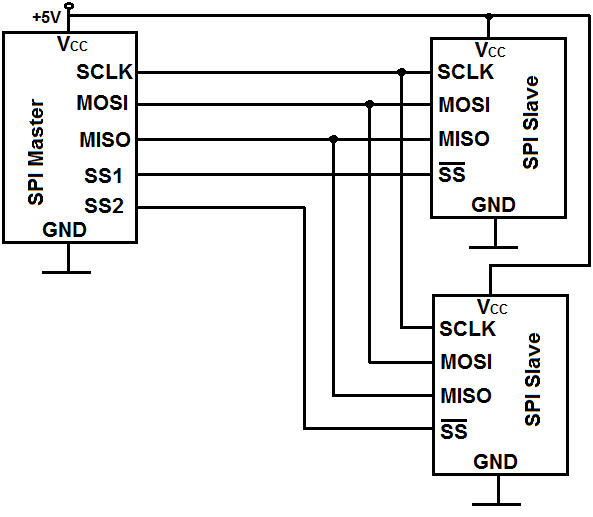
\includegraphics[width=0.55\linewidth]{Figures/SPI}
\caption[SPI configuration]{SPI configuration}
\label{spi}
\end{figure}
\end{center}
In this configuration the when the chip select pin of an amplifier is set to low, the microcontroller is able to obtain data from that strain gauge. This configuration allows for a four wire interface to connect to six strain gauge sensors and obtain measurements.

The HX711 however allows for the I2C like communication via two wires (serial clock (SCL) and Serial Data (SDA)). They however do not have hardware addresses thus many pins are required for the interface, This can however be remedied by the use of a shared SCL between each of the amplifier modules reducing the overall number of pins required to interface.

\subsection{Software and Control}
This section deals with the control of the stewart platform. It involves allowing input and obtaining output form the platform force balance.
\subsubsection{Human Machine Interface}
The purpose of the interface is to enable control of the platform position as well as to obtain measured data from the strain gauges and pitot tubes. 
The general layout is as shown in the figure \ref{fig:hmi}:
\begin{center}
\begin{figure}[H]
\centering
\includegraphics{Figures/Interface}
\caption[Human Machine Interface]{Human Machine Interface}
\label{fig:hmi}
\end{figure}
\end{center}

The primary interface between the microcontroller is wireless. 
For this interface two transport methods were considered: User Datagram Protocol (UDP) and Transmission Control protocol (TCP).
UDP is a communications protocol that is primarily used to establish low-latency and loss-tolerating connections.
 TCP on the hand does not experience data loss and in our case the use of protocol buffers as a means of serialization of messages to binary saving on bandwidth. 
 TCP requires only one initial handshake between the server and client, after which messages can be transmitted continuously (streaming).
 Due to assurance of data integrity (no loss) and lower bandwidth use thus higher data transfer rates, TCP was chosen as the main protocol.
  This allows for high speed low latency communication without need for a wired connection. It also allows for bidirectional streaming of information thus allowing for both control input and output of measured values. The interface is to enable the abstraction of data acquisition and actuator control to a simple interaction with buttons and other visual interfaces available in a computer program.
The decoupling of the microcontroller and the program to be hosted on the desktop allows for advanced data processing such as application of filters and resolving measurements into usable information. It also allows for the use of more powerful processor and high level programming languages to more effectively perform complex calculations without taking a toll the sensor sampling rate that would occur with on board processing in the microcontroller.

A user interface was also required to record user input and display incoming data.
\subsubsection{Control Algorithm}
\begin{center}
	\begin{figure}[H]
	\centering
	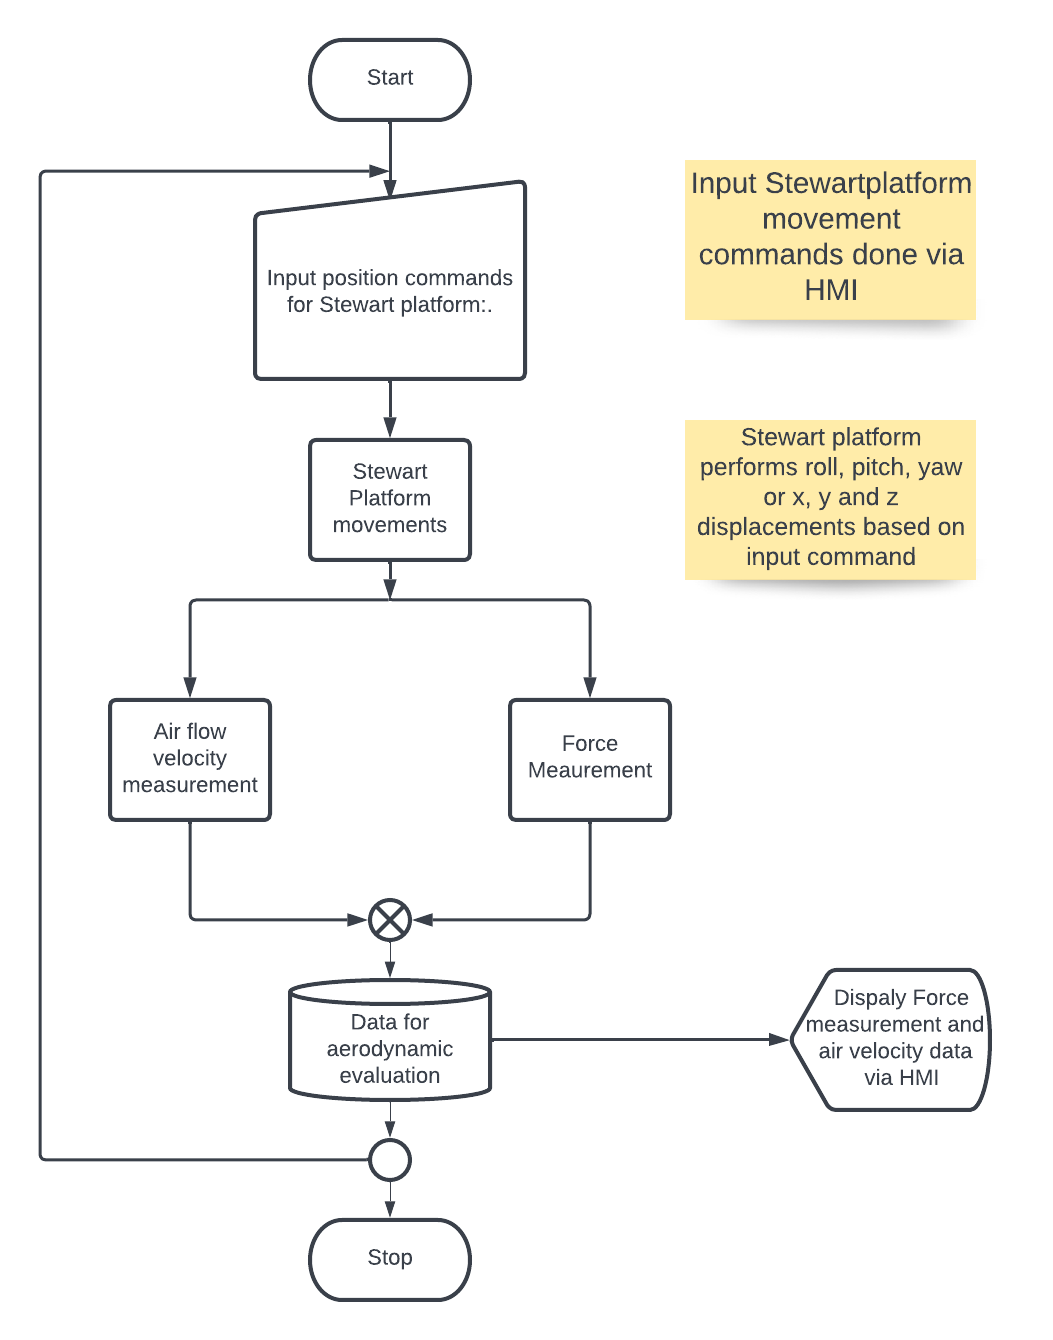
\includegraphics[width=0.7\linewidth]{Figures/Flow}
	\caption[Control Algorithm]{Control Algorithm for the Stewart Platform with Force Measurement}
	\end{figure}
\end{center}